\subsection{Overview}
 Here the architectural elements that compose the system are explained with their interaction. A description of the replication mechanism chosen in order to make the system distributed is also given.
The architectural framework adopted by the CKB platform needs to be robust and scalable. A three-tier application model is used, since it guarantees several of the nonfunctional requirements previously described in the RASD, such as reliability, since having several components which perform the same activity renders the system fault-tolerant, and maintainability, because having a system divided into three layers, any of which independent from the other ones, ensures atomicity between their functionalities. In addition, each tier runs on its own infrastructure, so can be developed individually and simultaneously with the others, giving flexibility and scalability to the system.
This architectural paradigm consists of three tiers: the presentation tier, the application logic tier, and the data storage tier.

\begin{figure}[H]
    \centering
    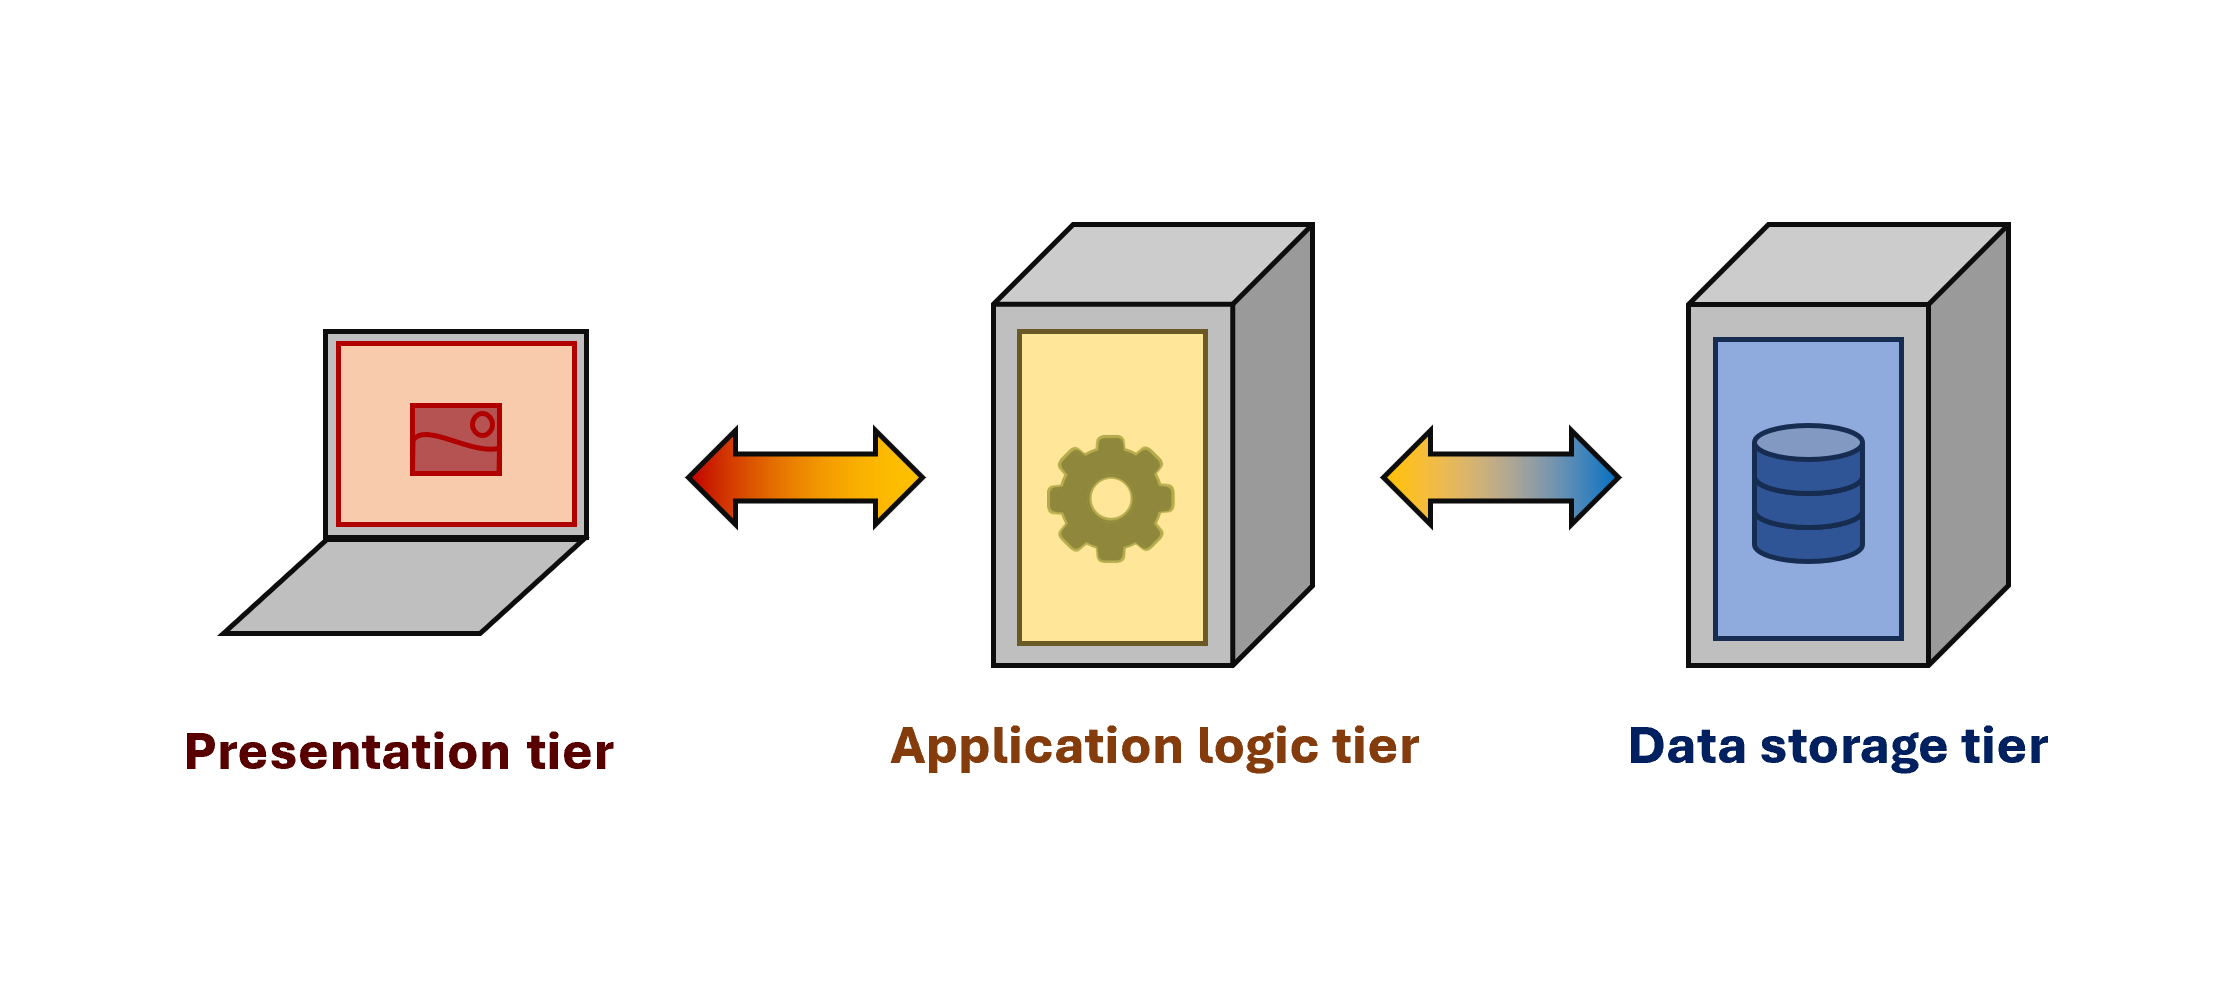
\includegraphics[width=0.9\linewidth]{Images/Threetiers.png}
    \caption{Visual representation of a three-tier architecture}
    \label{fig:enter-label}
\end{figure}

\begin{enumerate}
\item \textbf{Presentation Tier:} its functions are providing the user interface, and handling user interactions. This tier is client side and interacts directly within users' browsers. All web-based interfaces are executed on the client-side, allowing educators and students to interact with the CKB platform. Since the computation is done locally on the client, the user experience will be efficient and responsive.
\item \textbf{Application Logic Tier:} it’s positioned on the server-side, and its function is encapsulating the core functionalities of the CKB platform.  It contains the business logic, the code execution engines, facilitating communication between the users and the system. 
\item \textbf{Data Storage Tier:} it's on server-side and it's the foundation of the architecture, where platform’s relational databases store, manage and retrieve all necessary information. To optimize data accessibility and ensure data integrity, a database management system (DBMS) is employed. For security measures, encrypted connections and access controls are implemented, to safeguard users’ sensitive information and system data, and against unauthorized access and data breaches.
\end{enumerate}
The CKB platform can be accessed only via web browser, which interacts with the presentation tier. On the server side there are two components situated in the application tier (application server and web server) and one component situated in the data tier (database server). The web server handles the HTTP requests sent by browsers and returns the correct web pages in response, it also need to communicate with the application server via suitable API calls if, to satisfy such requests are necessary some data from the database, this because the web server and the DB are not directly connected.\\
The application server communicates with the database server that retrieves all the information about students, educators, battles, tournaments, badges, deadlines and so on from the DB. This because the application tier must be able to add, delete or modify data in the data tier using API calls. \\
In addition, the application server also needs to communicate with the GitHub Action service and Email Provider service (to send confirmation mail to registered users) via some API call, to provide the code written by teams to the system, that evaluates it and updates immediately the ranking.\\ \\
Since the system is distributed, so are the web servers, the application servers and the database servers, for this reason three load balancers are inserted into the architecture to dispatch the requests to web servers and application servers: all the requests coming from web browsers are captured by a load balancer that redirects the request to one of the web servers available to handle it. Then the web server manipulates the request and forwards it to the second load balancer, that dispatches requests from web servers to the application server that better elaborates the request in terms of time. \\ \\
The DBMS should be clustered so that consistency is guaranteed, and the performances are sufficient to fulfill a large number of queries in a reasonable time. The replicated database servers' main function is manage all data relevant to the application. The third load balancer is interposed between application servers and database servers. \\ \\
To guarantee a good level of security, a firewall is installed between every tier and between the external network (internet) and the internal network. Its functionalities are monitor, filter, and control incoming and outgoing network traffic based on predetermined and personalized security rules; it works as barriers between a trusted internal network and untrusted external networks that control the flow of traffic and prevent unauthorized access, protecting against various cyber threats and attacks. For other security measures, a Web Application Firewall (WAF) and an Intrusion Detection System (IDS) are integrated into the application tier, the first is necessary to safeguard against common web application threats and enhance overall security, while the second monitors and analyzes system activities, detecting and responding to suspicious behavior that may compromise the platform's integrity. Finally, the Demilitarized Zone (DMZ) is a network segment designed to provide an additional layer of security by placing certain services that need to be accessible from the internet in an isolated zone separate from the internal network, it acts as a buffer zone between the untrusted external network and the trusted internal one; its creation in our architecture is crucial to avoid the whole collapse of the system in case of malicious attacks, giving the possibility to isolate the cause of the attack to a specific component.\\ \\
In the following sections there is a presentation about the components of the systems and their interactions, completed with diagrams and schemas. Then, given the description of the components and their characteristics is presented an exhaustive discussion concerning the runtime specifications of the system with the use of sequence diagrams. Finally, dependency analysis of the component interfaces is shown.

\newpage

\begin{figure}[H]
    \centering
    {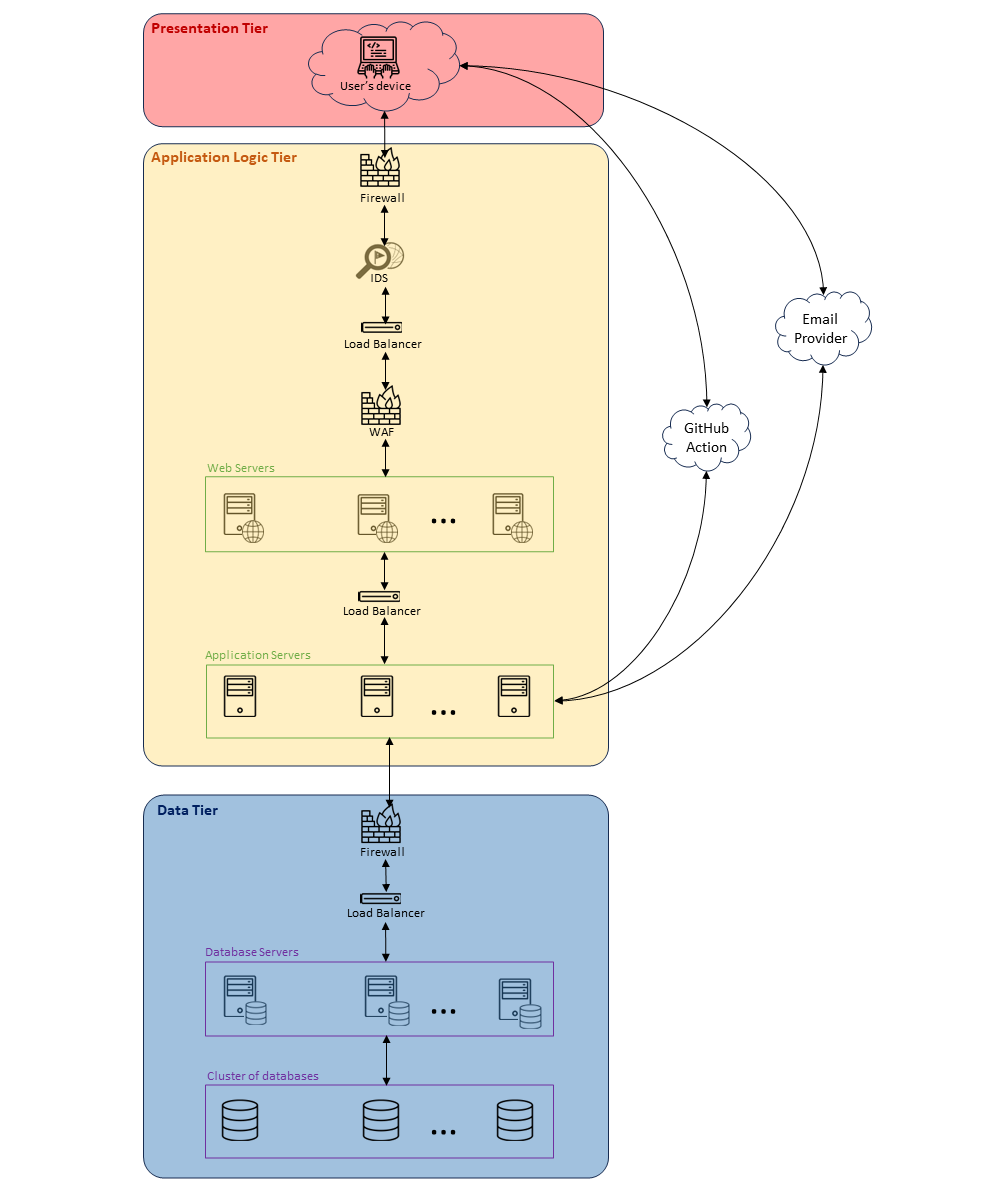
\includegraphics[width=1.2\linewidth]{Images/Architecture.png}}
    \caption{System Architecture}
    \label{fig:system_architecture}
\end{figure}

\newpage
 
\subsection{Component View}


\begin{figure}[H]
    \centering
    \rotatebox{-90}{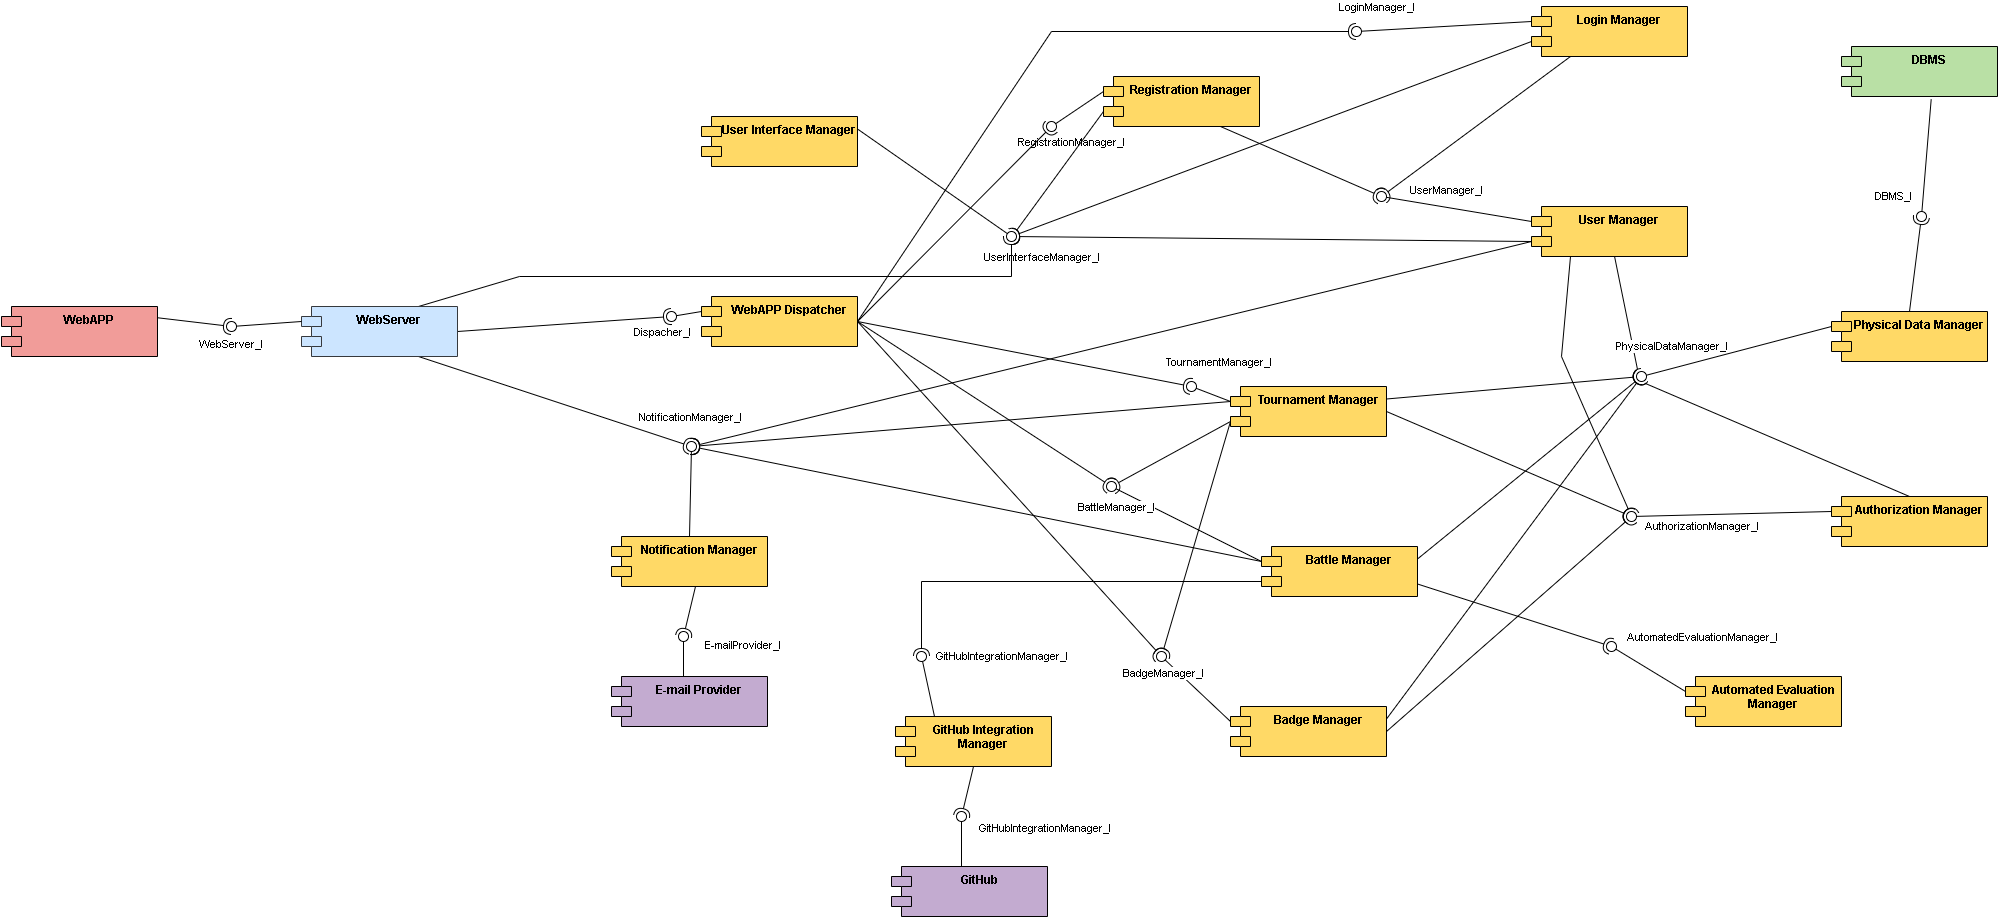
\includegraphics[width=1.35\linewidth]{Images/ComponentDiagram.png}}
    \caption{Component diagram}
    \label{fig:component_diagram}
\end{figure}

\begin{itemize}

    \item \textbf{Web App Dispatcher:} \\
Handles the incoming requests, forwarding them to the correct component in order to subdivide the workload and correctly elaborate each request.

    \item \textbf{User Manager:} \\
Handles students and educators' data such as login parameters, profile description, badges, and more.

    \item \textbf{Registration Manager:} \\
Handles user registration process. Checks the validity of the inserted data and stores it in a secure manner.

    \item \textbf{Login Manager:} \\
Handles user login and authentication processes, keeping track of unusual behaviours and correctly handling sensitive data.

    \item \textbf{Authorization Manager:} \\
Handles user authorization processes.
Manages user roles (Students, Educators) and their respective permissions.

    \item \textbf{Tournament Manager:}  \\
Manages the creation, updating, and closure of tournaments.
Includes components for handling registrations and scoring.

    \item \textbf{Battle Manager:}  \\
Manages the creation, updating, and closure of battles.
Includes components for handling registrations, submissions, and scoring.

    \item \textbf{GitHub Integration Manager:} \\
Facilitates the integration with GitHub for repository creation, forking, and workflow setup.
Manages the communication between the CKB platform and GitHub.

\item \textbf{Automated Evaluation Manager:}\\
Handles the automated evaluation of code submissions during battles.
Integrates with build automation and testing tools.

\item \textbf{User Interface (UI) Manager:} \\
    Responsible for presenting information to users and capturing their interactions. Includes components for displaying tournament and battle information, user profiles, and submission interfaces.

\item \textbf{Badge Manager} \\
Manages the creation and assignment of badges within the context of tournaments.
Handles the association of badges with specific rules and user achievements.

\item \textbf{Notification Manager:} \\
Manages the generation and delivery of notifications to users about new tournaments, battles, and closures.

\item \textbf{Physical Data Manager:} \\
Stores and retrieves data related to users, tournaments, battles, submissions, and other relevant information. It is responsible for the communication with the DBMS.
\end{itemize}


\subsection {Deployment View}

\begin{figure}[H]
    \centering
    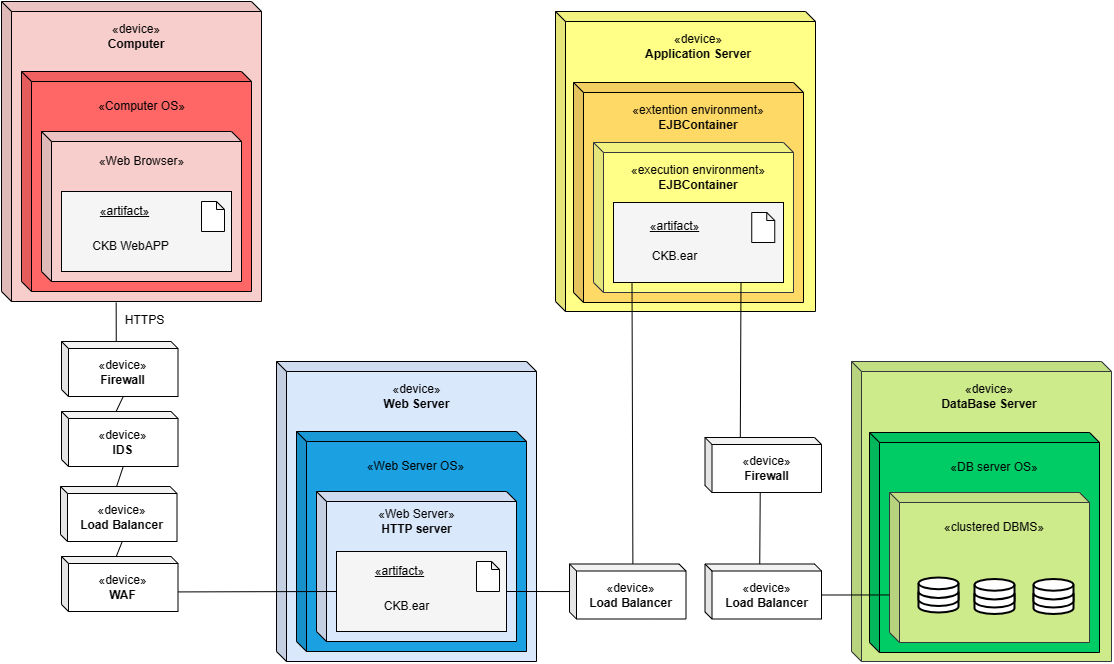
\includegraphics[width=1\linewidth]{Images/DeploymentView.png}
    \caption{Enter Caption}
    \label{fig:enter-label}
\end{figure}

\begin{itemize}
    \item Web Server:
    \item Application Server:
    \item Database Server:
    \item Load Balancer:
    \item GitHub Server:
    \item Client Devices (Computers with Web Browsers):
    \item E-mail Provider:
\end{itemize}

\subsection{Runtime View}
 You can use sequence diagrams to describe the way components interact to accomplish specific tasks typically related to your use cases.

 \begin{itemize}
    \item User Registration:
    \item User Login:
    \item Creating a Tournament:
    \item Student Joining a Battle:
    \item Automated Workflow Setup on GitHub:
    \item Real-Time Score Update:
    \item Manual Evaluation by Educator:
    \item Tournament Closure and Badge Assignment:
\end{itemize}

 \subsection{Component Interfaces}

 \subsection{Selected Architectural Styles and Patterns}
Please explain which styles/patterns you used, why, and how 
\begin{itemize}
    \item 3-tier Architecture: \\
    brief description
    \item MVC 
    \item  Facade pattern
    \item Mediator pattern
    \item others...
\end{itemize}

\subsection{Other Design Decisions}
\begin{itemize}
    \item availability
    \item notification timed
    \item  data storage
\end{itemize}